% =====================================================================
%  GEN3D -- FYP-1 Report (40% modules)
%  Compile: pdflatex main -> bibtex main -> pdflatex main -> pdflatex main
%  (or upload the whole docs/report folder to Overleaf)
%  Fill in the placeholders in the "Project details" block below.
% =====================================================================
\documentclass[12pt,a4paper]{report}

\usepackage[utf8]{inputenc}
\usepackage[T1]{fontenc}
\usepackage{lmodern}
\usepackage[margin=1in]{geometry}
\usepackage{graphicx}
\usepackage{booktabs}
\usepackage{tabularx}
\usepackage{amsmath,amssymb}
\usepackage{algorithm}
\usepackage{algpseudocode}
\usepackage{xcolor}
\usepackage{tikz}
\usetikzlibrary{arrows.meta,positioning,fit,backgrounds}
\usepackage{enumitem}
\usepackage{caption}
\usepackage{float}
\usepackage{listings}
\usepackage[hidelinks]{hyperref}
\usepackage{setspace}
\onehalfspacing

\graphicspath{{figures/}}
\lstset{basicstyle=\ttfamily\small,breaklines=true,frame=single,columns=fullflexible}

% ---------------- Project details (fill in) ----------------
\newcommand{\projecttitle}{GEN3D: Single-Image to Low-Poly, Texture-Preserved 3D Mesh Generation}
\newcommand{\studentA}{Student Name 1 (Reg. No.)}
\newcommand{\studentB}{Student Name 2 (Reg. No.)}
\newcommand{\studentC}{Student Name 3 (Reg. No.)}
\newcommand{\supervisor}{Supervisor Name}
\newcommand{\degree}{Bachelor of Science in Computer Science}
\newcommand{\university}{National University of Computer and Emerging Sciences, Peshawar Campus}
\newcommand{\reportdate}{November 2026}
\newcommand{\todo}[1]{\textcolor{red}{[TODO: #1]}}
% ------------------------------------------------------------

\begin{document}

% ---------------- Title page ----------------
\begin{titlepage}
  \centering
  {\large \university\par}
  \vspace{2.5cm}
  {\LARGE\bfseries \projecttitle\par}
  \vspace{1cm}
  {\large Final Year Project -- Part I Report (40\% modules)\par}
  \vspace{2cm}
  {\large \studentA\\ \studentB\\ \studentC\par}
  \vspace{1.5cm}
  {\large Supervisor: \supervisor\par}
  \vfill
  {\large \degree\par}
  \vspace{0.5cm}
  {\large \reportdate\par}
\end{titlepage}

\pagenumbering{roman}

\chapter*{Abstract}
\addcontentsline{toc}{chapter}{Abstract}
Three-dimensional (3D) assets are central to games, augmented and virtual reality, and online retail, yet producing them by hand is slow and expensive. Recent image-to-3D methods can create a mesh from a single photograph, but they produce dense meshes with tens to hundreds of thousands of faces, which are too heavy for real-time use. Standard mesh simplification such as Quadric Error Metrics (QEM)~\cite{garland1997qem} reduces the face count but ignores the texture, so colours stretch and tear along UV seams.

GEN3D addresses both problems in one pipeline. A generator that we design and train ourselves turns one photograph into a textured 3D mesh. It combines a pretrained DINOv2 encoder~\cite{oquab2023dinov2} with pixel-aligned features~\cite{saito2019pifu,xu2019disn}, an occupancy decoder~\cite{mescheder2019onet} and a texture field~\cite{oechsle2019texturefields}. The resulting high-poly mesh is then simplified by a texture-aware QEM and, as the main contribution of the project, by D-QEM, in which a Transformer~\cite{vaswani2017attention} learns a correction to the QEM collapse cost that accounts for UV seams, UV stretch and colour change.

This report covers the first 40\% of the project. We built a class-agnostic dataset of 7{,}467 clean objects from 1{,}028 categories of Objaverse-LVIS~\cite{deitke2023objaverse}, wrote our own inside/outside labelling method for non-watertight meshes, rendered 16 calibrated views per object with Blender, automated all heavy computation on Kaggle GPUs, and implemented and verified the generator. The texture-aware QEM, the D-QEM Transformer and the interactive demo follow in the remaining modules.


\tableofcontents
\listoffigures
\listoftables

\clearpage
\pagenumbering{arabic}

\chapter{Introduction}

\section{Background and Need}
Games, AR/VR applications and e-commerce product viewers all depend on 3D models. Each model must look right, which means accurate shape and a sharp texture, and it must be light, meaning a low polygon count, so that it renders in real time on phones and headsets. Creating such assets by hand requires skilled artists and hours of work per object.

Single-image 3D reconstruction promises to automate this step: a user photographs an object and receives a 3D model. Current methods, however, output dense meshes of roughly 50{,}000 to 200{,}000 faces. Reducing these meshes with conventional simplification damages their textures, because the simplification only measures geometric error.

\section{Motivation: What If We Do Not Do This Project?}
Without a tool like GEN3D, small studios, students and online sellers must either pay for manual modelling or accept heavy meshes that are slow on mobile devices. If they simplify those meshes with standard tools, they get visible texture tearing along seams. GEN3D aims to give them a light, good-looking asset from one photograph.

\section{Problem Statement}
Given a single RGB image of an object, produce a low-poly 3D mesh whose geometry and texture remain faithful to the object. Existing image-to-3D models produce high-poly meshes, and existing simplification methods reduce polygons without accounting for texture, so no available pipeline delivers both low polygon count and preserved texture from a single image.

\section{Proposed Solution}
GEN3D is a two-stage pipeline:
\begin{enumerate}[leftmargin=*]
  \item \textbf{Generator (image $\rightarrow$ textured high-poly mesh).} An image-conditioned occupancy network trained by us: a DINOv2 encoder, pixel-aligned features, an occupancy decoder and a texture field. Marching cubes~\cite{lorensen1987marching} extracts the mesh.
  \item \textbf{Texture-aware simplification (high-poly $\rightarrow$ low-poly).} A QEM variant that includes UV coordinates in the quadric and locks UV seams~\cite{garland1998color}, extended by \textbf{D-QEM}, where a Transformer predicts an additional collapse cost:
  \begin{equation}
    \text{cost}(e) = \text{QEM}(e) + \lambda \cdot \text{Transformer}(e).
  \end{equation}
\end{enumerate}

\section{Goals}
\begin{itemize}[leftmargin=*]
  \item Generate a textured 3D mesh from one photograph with a model trained by the team.
  \item Reduce the mesh to 10--50\% of its faces while preserving texture quality better than standard QEM.
  \item Deliver an interactive demo in which a user uploads a photo and compares original and simplified meshes.
\end{itemize}

\section{Objectives}
\subsection{FYP-1 (40\%)}
\begin{enumerate}[leftmargin=*]
  \item Curate and preprocess a large, clean training dataset (done: 7{,}467 objects, 1{,}028 categories).
  \item Render calibrated multi-view images of every object (3{,}118 objects done, remainder scheduled).
  \item Implement and train the generator (implemented and verified; first full training run in progress).
  \item Implement the texture-aware QEM.
  \item Build a Gradio demo of the full pipeline.
  \item Produce design documents and this report.
\end{enumerate}
\subsection{FYP-2 (60\%)}
\begin{enumerate}[leftmargin=*]
  \item Train the D-QEM Transformer at full scale and evaluate it against QEM baselines.
  \item Add UV unwrapping and texture baking to generated meshes.
  \item Run full evaluation and ablation studies; finalise the demo and thesis.
\end{enumerate}

\section{Scope}
Input is a single RGB image of one object on a plain or removable background. Training uses Objaverse-LVIS only. Training is class-agnostic: the model receives no category label and learns general 3D structure. The demo focuses on four categories (chair, table, cup, cupboard). Scenes with many objects, transparent materials and articulated characters are out of scope.

\section{Expected Results}
At the end of the project a user uploads a photo of, for example, a chair. GEN3D shows a rotatable 3D model within seconds, and a slider reduces it to 10\% of its faces. Side by side, a standard tool's result shows torn or stretched texture, while GEN3D's result keeps the texture clean. A table under the models reports shape error (Chamfer distance) and texture error (LPIPS) for each method.

\chapter{Literature Review}

\section{3D Representations}
A learning system must choose how to represent 3D output. \emph{Voxels} are a regular 3D grid; memory grows cubically, so practical grids stay at $32^3$--$64^3$~\cite{choy2016r2n2}. \emph{Point clouds} are unordered sets of points without connectivity~\cite{fan2017psgn}. \emph{Meshes} are vertices and triangular faces, the format used by games and AR. \emph{Implicit functions} represent a shape as a function over 3D space, either occupancy~\cite{mescheder2019onet} or signed distance~\cite{park2019deepsdf}, and can be evaluated at any resolution. \emph{Radiance fields}~\cite{mildenhall2020nerf} and \emph{3D Gaussians}~\cite{kerbl2023gaussian} model appearance for photorealistic rendering.

\section{Single-Image 3D Reconstruction}
3D-R2N2~\cite{choy2016r2n2} predicted voxel grids and PSGN~\cite{fan2017psgn} predicted point clouds. Pixel2Mesh~\cite{wang2018pixel2mesh} deforms a template sphere into a mesh, which cannot create holes such as the gaps between chair legs. AtlasNet~\cite{groueix2018atlasnet} assembles surface patches that may self-intersect.

Occupancy Networks~\cite{mescheder2019onet} learn a function $f_\theta(p, x) \in [0,1]$ that gives the probability that point $p$ lies inside the object seen in image $x$. The surface is a level set of $f_\theta$ and is extracted with marching cubes~\cite{lorensen1987marching}. On ShapeNet single-image reconstruction ONet reported a mean IoU of 0.571, against 0.493 for 3D-R2N2 and 0.480 for Pixel2Mesh, and the best normal consistency (0.834). It conditions the decoder only on a global image feature, which blurs fine detail. PIFu~\cite{saito2019pifu} and DISN~\cite{xu2019disn} address this with \emph{pixel-aligned} features: each 3D point is projected into the image and the local feature at that pixel is used. Texture Fields~\cite{oechsle2019texturefields} predict colour as a function over the surface.

Large reconstruction models (LRM~\cite{hong2024lrm}, TripoSR~\cite{tochilkin2024triposr}, SF3D~\cite{boss2024sf3d}) use large Transformers and triplane representations trained on hundreds of thousands of objects with many GPUs. Diffusion-based methods such as Zero-1-to-3~\cite{liu2023zero123} first synthesise new views. These give the best quality but are far beyond the compute and data available to this project.

\section{Mesh Simplification}
QEM~\cite{garland1997qem} assigns each vertex a $4\times4$ quadric matrix accumulated from the planes of its adjacent faces. The cost of collapsing an edge is the quadric error at the new vertex position; edges are collapsed cheapest first using a priority queue. Garland and Heckbert extended quadrics to colour and texture coordinates~\cite{garland1998color}, and Hoppe proposed a more efficient appearance-attribute metric~\cite{hoppe1999newquadric}. Neural Mesh Simplification~\cite{potamias2022nms} learns to select points and triangles directly, but does not model UV coordinates or texture.

\section{Comparison and Research Gap}
\begin{table}[H]
\centering
\caption{Comparison of related methods.}
\label{tab:related}
\small
\begin{tabularx}{\textwidth}{lXccc}
\toprule
Method & Idea & Image input & Textured output & Texture-aware low-poly \\
\midrule
3D-R2N2~\cite{choy2016r2n2} & Voxel grid & \checkmark & -- & -- \\
Pixel2Mesh~\cite{wang2018pixel2mesh} & Deform sphere & \checkmark & -- & -- \\
ONet~\cite{mescheder2019onet} & Occupancy function & \checkmark & -- & -- \\
PIFu / DISN~\cite{saito2019pifu,xu2019disn} & Pixel-aligned implicit & \checkmark & partial & -- \\
TripoSR / SF3D~\cite{tochilkin2024triposr,boss2024sf3d} & Large triplane model & \checkmark & \checkmark & -- \\
QEM~\cite{garland1997qem,garland1998color} & Quadric edge collapse & -- & keeps UVs & hand-made metric \\
Neural Mesh Simpl.~\cite{potamias2022nms} & Learned selection & -- & -- & -- \\
\textbf{GEN3D (ours)} & Occupancy + learned QEM & \checkmark & \checkmark & \checkmark \\
\bottomrule
\end{tabularx}
\end{table}

\paragraph{Gap.} Image-to-3D methods output heavy meshes, and simplification methods either ignore texture or rely on a fixed, hand-designed metric. No method in Table~\ref{tab:related} learns, from data, how much each edge collapse damages the texture, and none joins this to an image-to-3D generator. GEN3D fills this gap with D-QEM.

\paragraph{Note.} A focused search of 2023--2026 work on learned and texture-aware simplification is planned before the final novelty claim. \todo{update after literature search}

\chapter{Methodology}

\section{System Overview}
Figure~\ref{fig:pipeline} shows the GEN3D pipeline. Part A builds the training data once. Part B is the generator, trained on that data. Part C simplifies the generated mesh while keeping its texture. Part D is the demo.

\begin{figure}[H]
\centering
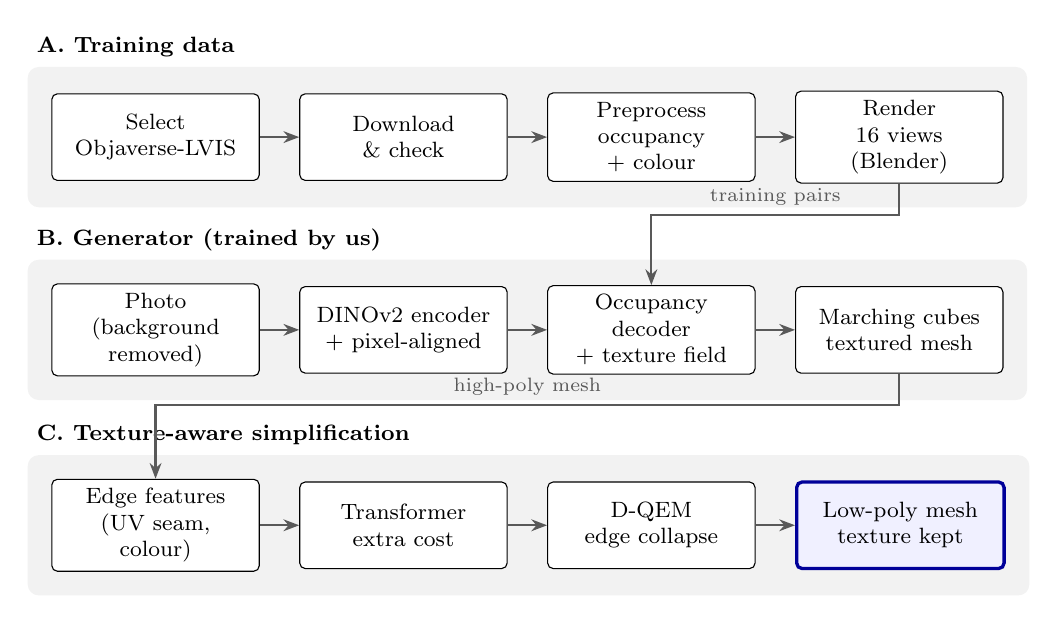
\begin{tikzpicture}[
  node distance=4mm and 5mm,
  box/.style={draw, rounded corners=2pt, align=center, font=\footnotesize, minimum height=11mm, text width=24mm, fill=white},
  key/.style={box, very thick, draw=blue!60!black, fill=blue!6},
  lane/.style={draw=none, fill=gray!10, rounded corners=4pt, inner sep=3mm},
  lab/.style={font=\footnotesize\bfseries, anchor=west},
  arr/.style={-{Stealth[length=2mm]}, thick, gray!70!black}]
  % lane A
  \node[box] (a1) {Select\\Objaverse-LVIS};
  \node[box, right=of a1] (a2) {Download\\\& check};
  \node[box, right=of a2] (a3) {Preprocess\\occupancy + colour};
  \node[box, right=of a3] (a4) {Render\\16 views (Blender)};
  % lane B
  \node[box, below=13mm of a1] (b1) {Photo\\(background removed)};
  \node[box, right=of b1] (b2) {DINOv2 encoder\\+ pixel-aligned};
  \node[box, right=of b2] (b3) {Occupancy decoder\\+ texture field};
  \node[box, right=of b3] (b4) {Marching cubes\\textured mesh};
  % lane C
  \node[box, below=13mm of b1] (c1) {Edge features\\(UV seam, colour)};
  \node[box, right=of c1] (c2) {Transformer\\extra cost};
  \node[box, right=of c2] (c3) {D-QEM\\edge collapse};
  \node[key, right=of c3] (c4) {Low-poly mesh\\texture kept};
  \begin{scope}[on background layer]
    \node[lane, fit=(a1)(a4)] (la) {};
    \node[lane, fit=(b1)(b4)] (lb) {};
    \node[lane, fit=(c1)(c4)] (lc) {};
  \end{scope}
  \node[lab] at ([yshift=2.5mm]la.north west) {A. Training data};
  \node[lab] at ([yshift=2.5mm]lb.north west) {B. Generator (trained by us)};
  \node[lab] at ([yshift=2.5mm]lc.north west) {C. Texture-aware simplification};
  \foreach \x/\y in {a1/a2,a2/a3,a3/a4,b1/b2,b2/b3,b3/b4,c1/c2,c2/c3,c3/c4} \draw[arr] (\x) -- (\y);
  \draw[arr] (a4.south) -- ++(0,-4mm) -| node[pos=0.25, above, font=\scriptsize]{training pairs} (b3.north);
  \draw[arr] (b4.south) -- ++(0,-4mm) -| node[pos=0.25, above, font=\scriptsize]{high-poly mesh} (c1.north);
\end{tikzpicture}
\caption{GEN3D pipeline: training data (A), generator (B) and texture-aware simplification (C).}
\label{fig:pipeline}
\end{figure}

\section{Dataset Construction}
\subsection{Source and Class-Agnostic Selection}
We use Objaverse~\cite{deitke2023objaverse}, a collection of about 800{,}000 3D models, restricted to its LVIS-annotated subset of 46{,}207 objects in 1{,}156 categories (LVIS vocabulary~\cite{gupta2019lvis}). Only 1{,}283 objects belong to our four demo categories, which is too few to train a generator. We therefore train \emph{class-agnostically}: the model never receives a category label and learns general 3D structure from many categories. The selection has three groups:
\begin{itemize}[leftmargin=*]
  \item \textbf{demo} -- every object of chair, table, cup and cupboard (and synonyms);
  \item \textbf{related} -- furniture, household items, toys and vehicles, sampled with five times the weight;
  \item \textbf{other} -- all remaining categories, taken round-robin so that every category contributes.
\end{itemize}
Forty whole categories from the \emph{other} group are held out as \texttt{test\_unseen} to measure generalisation to categories never seen in training.

\subsection{Filtering}
\begin{table}[H]
\centering
\caption{Filters applied before download (metadata) and after download (geometry).}
\label{tab:filters}
\small
\begin{tabularx}{\textwidth}{lX}
\toprule
Filter & Rule and reason \\
\midrule
Face count & 300--500{,}000: excludes trivial boxes and very heavy files \\
File size & $\le$ 60\,MB for demo, $\le$ 10\,MB otherwise: 224\,px renders do not need 4K textures; reduced download from 81\,GB to 28\,GB \\
Animation & excluded: mostly rigged characters \\
Name blacklist & scene, room, set, pack, collection, interior, bundle \\
Category blacklist & people, plants, clothing, glass, buildings, ropes, etc. \\
Mesh check & file must load and contain triangles; bounding-box aspect $\le 50$; ground plates flagged for review \\
Occupancy flags & bulky object with $<0.5\%$ interior (hollow), $>60\%$ interior (enclosing dome), or colourless \\
\bottomrule
\end{tabularx}
\end{table}

\subsection{Normalisation}
Every object is centred at its bounding-box centre and scaled so that its longest side equals 1, placing it inside $[-0.5, 0.5]^3$. The centre and scale are stored in \texttt{norm.json} and reused by the renderer, so images and 3D labels share one coordinate frame.

\section{Occupancy Labels for Non-Watertight Meshes}
Training an occupancy network requires knowing whether a 3D point lies inside the object. Objaverse meshes are rarely watertight: a chair seat is often a single open surface. We therefore wrote our own labelling method (Algorithm~\ref{alg:occ}), following the idea behind watertight conversion tools but without native dependencies, since \texttt{mesh2sdf} could not be built on our Windows machines.

\begin{algorithm}[H]
\caption{Occupancy labelling by flood fill}
\label{alg:occ}
\begin{algorithmic}[1]
\Require normalised mesh $M$, grid resolution $R=256$, skin $\ell = 0.9$ voxel
\State $S \gets$ 2{,}000{,}000 points sampled uniformly on the surface of $M$
\State build a KD-tree on $S$
\State $W \gets$ voxels whose centre lies within $\ell$ of $S$ \Comment{walls without gaps}
\State $E \gets$ flood fill of non-wall voxels starting from the grid border \Comment{exterior}
\For{each query point $p$}
  \State $d \gets$ distance from $p$ to nearest point of $S$ (bounded search)
  \If{$d < \ell$} \State inside$(p) \gets$ true \Comment{within the skin}
  \ElsIf{voxel$(p) \in E$} \State inside$(p) \gets$ false
  \Else \State inside$(p) \gets$ not ($p$ + 1.5 voxel away from the surface $\in E$)
  \EndIf
\EndFor
\end{algorithmic}
\end{algorithm}

The result is the watertight outer skin of the object, inflated by only 0.4\% of its size; thin parts become thin solid plates. Per object we store 100{,}000 labelled points (40\% near the surface with $\sigma=0.005$, 30\% with $\sigma=0.02$, 30\% uniform in the box) and 50{,}000 surface points with normals and colours read from the texture through the UV map.

\section{Multi-View Rendering}
Objaverse provides 3D models, not photographs. We create training images with Blender: a virtual camera views each object from 16 random directions (azimuth $0$--$360^\circ$, elevation $-10^\circ$ to $40^\circ$, distance 1.8--2.2) under randomised sun lighting, at $224\times224$ pixels with a transparent background. For every view we store the camera-to-world matrix and the intrinsic matrix $K$. Projecting the stored 3D surface points with these cameras places 100\% of them on the rendered object (Figure~\ref{fig:camera}), which confirms that images and labels are aligned.

\section{Generator: GEN3D-Gen}
\subsection{Architecture}
\begin{itemize}[leftmargin=*]
  \item \textbf{Encoder}: DINOv2 ViT-S/14~\cite{oquab2023dinov2,dosovitskiy2021vit}, pretrained. A $224\times224$ image gives a global feature and a $16\times16$ patch feature map, both projected to 256 channels. The first 8 of 12 Transformer blocks are frozen; the last 4 are fine-tuned.
  \item \textbf{Pixel-aligned features}~\cite{saito2019pifu,xu2019disn}: each query point $p$ is projected with the camera, $u = f_x x/(-z) + c_x$, $v = c_y - f_y y/(-z)$, and the feature map is sampled bilinearly at $(u,v)$.
  \item \textbf{Occupancy decoder}~\cite{mescheder2019onet}: a residual MLP (5 blocks, width 256) that maps the positional encoding of $p$, the global feature and the local feature to an inside logit.
  \item \textbf{Texture field}~\cite{oechsle2019texturefields}: a second residual MLP with the same inputs that outputs RGB.
\end{itemize}
The model has about 9.0 million trainable parameters.

\subsection{View-Centric Training}
Objaverse objects have arbitrary orientations. We express every target in the camera's frame: points are rotated by the camera rotation, so the network always predicts the shape as seen from the input view, and the original orientation of the object does not matter.

\subsection{Loss and Optimisation}
\begin{equation}
\mathcal{L} = \mathrm{BCE}\big(f_\theta(p, x), o(p)\big) + \lambda_{\text{tex}} \, \big\lVert c_\theta(s, x) - c(s) \big\rVert_1 ,
\end{equation}
where $o(p)$ is the occupancy label of point $p$ and $c(s)$ the colour of surface point $s$. Each sample uses 2{,}048 occupancy points and 1{,}024 colour points. We use AdamW with learning rate $10^{-4}$ for the decoders and $10^{-5}$ for the encoder, batch size 16 and mixed precision. To stop the largest category (chair) from dominating, objects are sampled with weight $1/\sqrt{n_c}$, where $n_c$ is the size of the object's category.

\subsection{Mesh Extraction}
The decoder is queried on a $128^3$ grid; marching cubes~\cite{lorensen1987marching} extracts the surface and the texture field colours its vertices. UV unwrapping with xatlas~\cite{xatlas} and texture baking are planned.

\section{Texture-Aware Simplification}
\subsection{QEM with UV and Seam Locking}
Following~\cite{garland1997qem,garland1998color}, each vertex keeps a quadric over position and UV coordinates. Edges are collapsed cheapest first using a min-heap; edges on UV seams are locked or heavily penalised so that the texture does not tear.

\subsection{D-QEM (planned)}
For each edge we compute features: length, sharpness, dihedral angle, boundary flag, QEM error, UV seam flag, UV stretch, colour variance, valence and curvature. A small MLP turns them into tokens, and a Transformer encoder~\cite{vaswani2017attention} over patches of 256--512 neighbouring edges predicts an extra cost. The training label is the measured damage of collapsing that edge alone (geometric plus texture error) minus its QEM cost, so the network learns only what QEM misses. Setting $\lambda=0$ recovers plain QEM, which makes ablation straightforward.

\chapter{Implementation}

\section{Technology Stack}
\begin{table}[H]
\centering
\caption{Technologies used.}
\small
\begin{tabularx}{\textwidth}{lX}
\toprule
Area & Tools \\
\midrule
Language & Python 3.11 \\
Data & Objaverse API, pandas \\
3D processing & trimesh~\cite{trimesh}, NumPy, SciPy (KD-tree, flood fill), scikit-image (marching cubes) \\
Rendering & Blender 4.2 LTS~\cite{blender}, Cycles on GPU \\
Learning & PyTorch~\cite{paszke2019pytorch}, timm (DINOv2) \\
Simplification & own QEM implementation; PyMeshLab as baseline only \\
Demo & Gradio, rembg \\
Compute & Kaggle notebooks (4-core CPU, 2$\times$ NVIDIA T4 GPU), Kaggle API \\
Version control & Git, GitHub \\
\bottomrule
\end{tabularx}
\end{table}

\section{Code Structure}
\begin{table}[H]
\centering
\caption{Main modules.}
\small
\begin{tabularx}{\textwidth}{lX}
\toprule
Path & Responsibility \\
\midrule
\texttt{configs/default.yaml} & every setting (filters, grid size, model, training); no hard-coded values \\
\texttt{gen3d/data/mesh\_io.py} & load GLB, normalise, sample coloured surface points \\
\texttt{gen3d/data/occupancy.py} & occupancy labelling (Algorithm~\ref{alg:occ}) \\
\texttt{gen3d/data/dataset.py} & PyTorch dataset: image, camera, points; $1/\sqrt{n}$ sampler \\
\texttt{gen3d/generator/encoder.py} & DINOv2 encoder (ResNet-18 kept for ablation) \\
\texttt{gen3d/generator/model.py} & generator, loss, IoU \\
\texttt{gen3d/generator/extract.py} & mesh extraction \\
\texttt{scripts/*.py} & pipeline steps: select, download, check, preprocess, render, review, train, generate \\
\texttt{kaggle/} & builds and pushes the Kaggle notebooks (data, render, train) \\
\bottomrule
\end{tabularx}
\end{table}

\section{Cloud Execution on Kaggle}
The laptop has no GPU, so all heavy work runs on Kaggle and is controlled from the laptop through the Kaggle API: the code is uploaded as a private dataset, each step is pushed as a notebook, and outputs are downloaded for inspection. Each notebook processes objects in chunks, saves every finished chunk immediately, stops before Kaggle's 12-hour limit, and resumes from where it stopped. The data notebook downloads, checks and preprocesses objects; the render notebook installs Blender, re-downloads each chunk of models, renders them with several Blender processes on two GPUs and stores each object's views as one zip file; the training notebook reads the outputs of both.

\section{Coding Conventions}
\begin{itemize}[leftmargin=*]
  \item Modular package (\texttt{gen3d/}) separated from runnable steps (\texttt{scripts/}).
  \item All parameters in one YAML configuration file.
  \item Docstrings on every module and function; descriptive names.
  \item Core algorithms (occupancy labelling, QEM, metrics) implemented by the team rather than taken from libraries.
  \item Every step is resumable and logs its decisions to CSV files, which also serve as the data dictionary.
\end{itemize}

\chapter{Results So Far}

\section{Dataset}
\begin{table}[H]
\centering
\caption{Dataset funnel.}
\label{tab:funnel}
\begin{tabular}{lr}
\toprule
Stage & Objects \\
\midrule
Objaverse-LVIS objects considered & 46{,}207 \\
Passed metadata filters & 25{,}441 \\
Selected (class-agnostic) & 8{,}000 \\
Passed mesh checks & 7{,}630 \\
\textbf{Clean after preprocessing} & \textbf{7{,}467} (1{,}028 categories) \\
\bottomrule
\end{tabular}
\end{table}

\begin{table}[H]
\centering
\caption{Clean objects per group and split.}
\label{tab:groups}
\begin{tabular}{lrr@{\hspace{2em}}lr}
\toprule
Group & Objects & Categories & Split & Objects \\
\midrule
demo & 1{,}212 & 4 & train & 5{,}833 \\
related & 855 & 32 & val & 715 \\
other & 5{,}400 & 992 & test & 702 \\
 & & & test\_unseen & 217 \\
\bottomrule
\end{tabular}
\end{table}
Demo categories: chair 566, table 230, cup 208, cupboard 208. Of the 8{,}000 selected objects, 314 were flagged for having a ground plate, 56 had degenerate geometry, and 163 were flagged during preprocessing (128 hollow, 24 colourless, 11 enclosed). Preprocessing took 4.3\,h on a 4-core Kaggle CPU.

\section{Preprocessing Quality}
Figure~\ref{fig:preprocess} shows, for several objects, the coloured surface samples, the points labelled inside and the extracted watertight surface. Thin legs and the open cavity of a cup are recovered correctly. Near-surface inside ratios dropped from about 0.9 with our first voxel shell to 0.43--0.70 after switching to exact distances, which matches the expected value for a 0.4\% skin.

\begin{figure}[H]
\centering
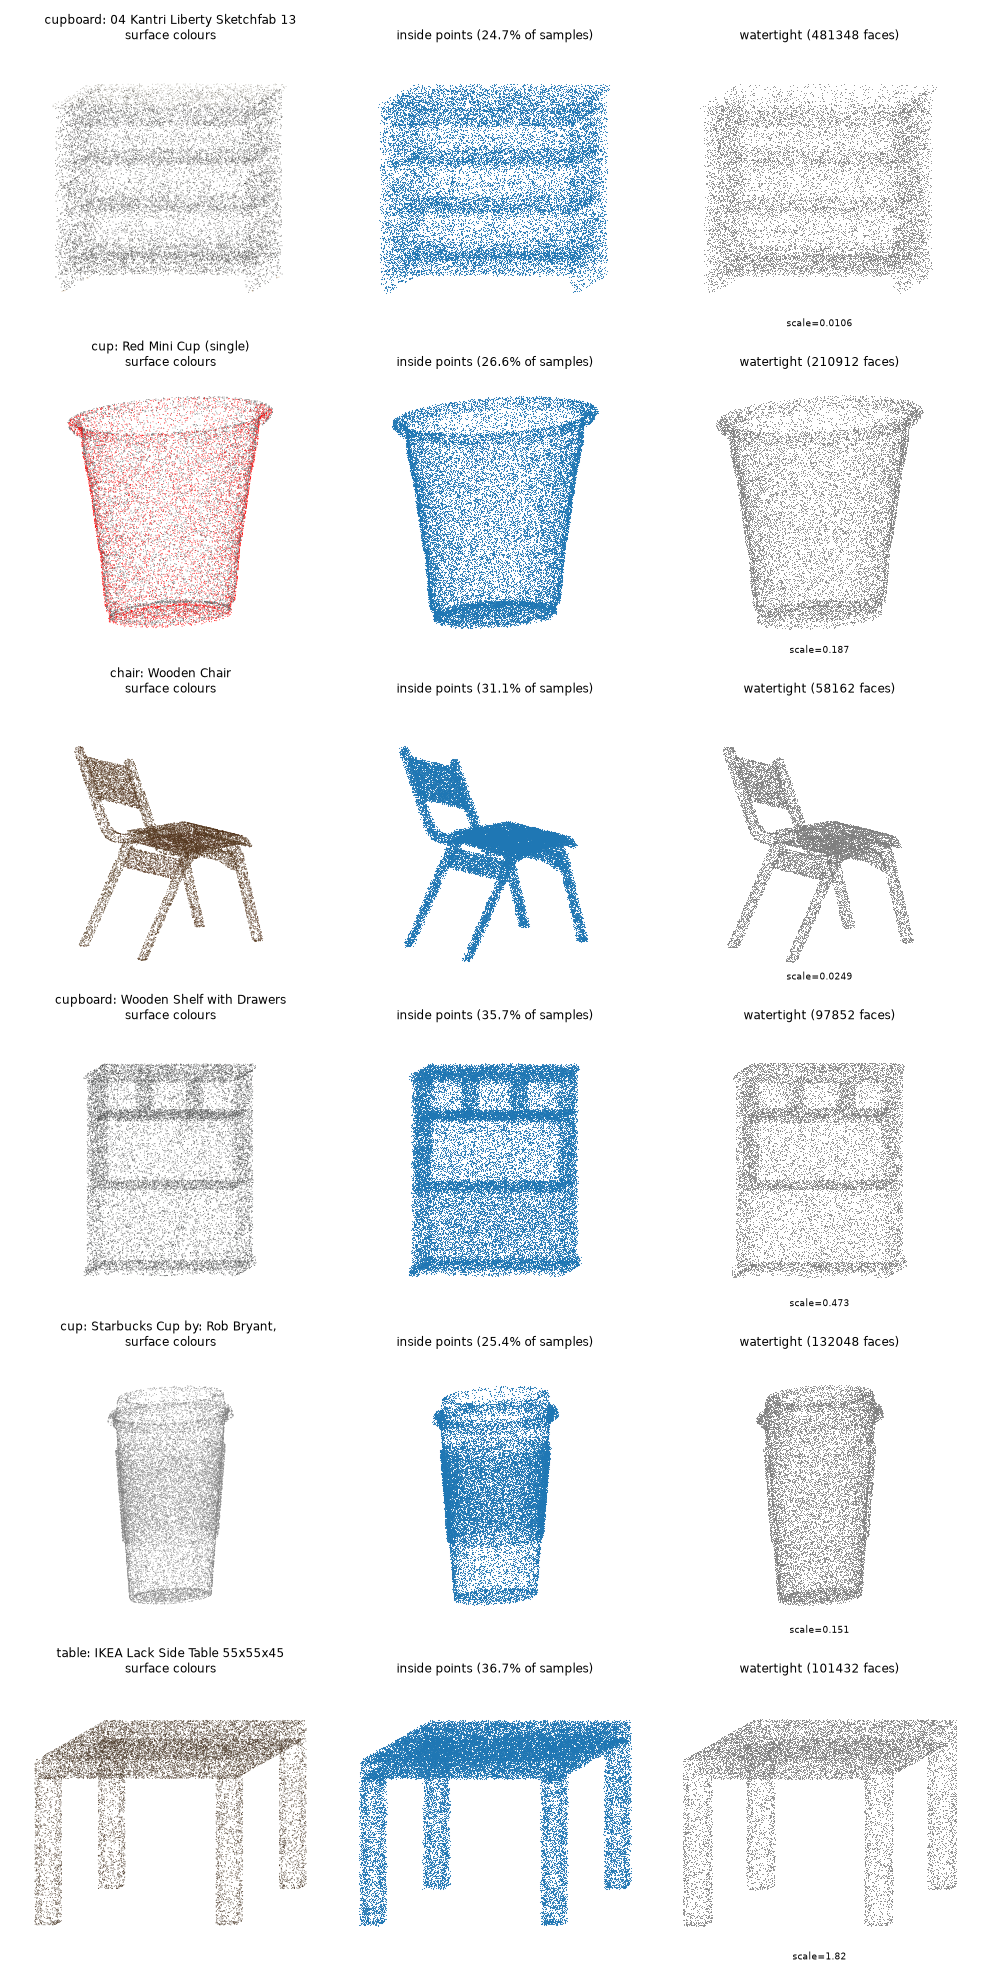
\includegraphics[width=0.75\textwidth]{preprocess_check.png}
\caption{Preprocessing output: surface colours, inside points and watertight surface.}
\label{fig:preprocess}
\end{figure}

\section{Rendering}
The first render run (16 views, 32 samples, two T4 GPUs) produced views for 3{,}118 objects in 11.95\,h at about 13.5\,s per object, covering every demo and related object. 82 objects failed and are scheduled for re-rendering. Figure~\ref{fig:renders} shows sample renders and Figure~\ref{fig:camera} the camera check.

\begin{figure}[H]
\centering
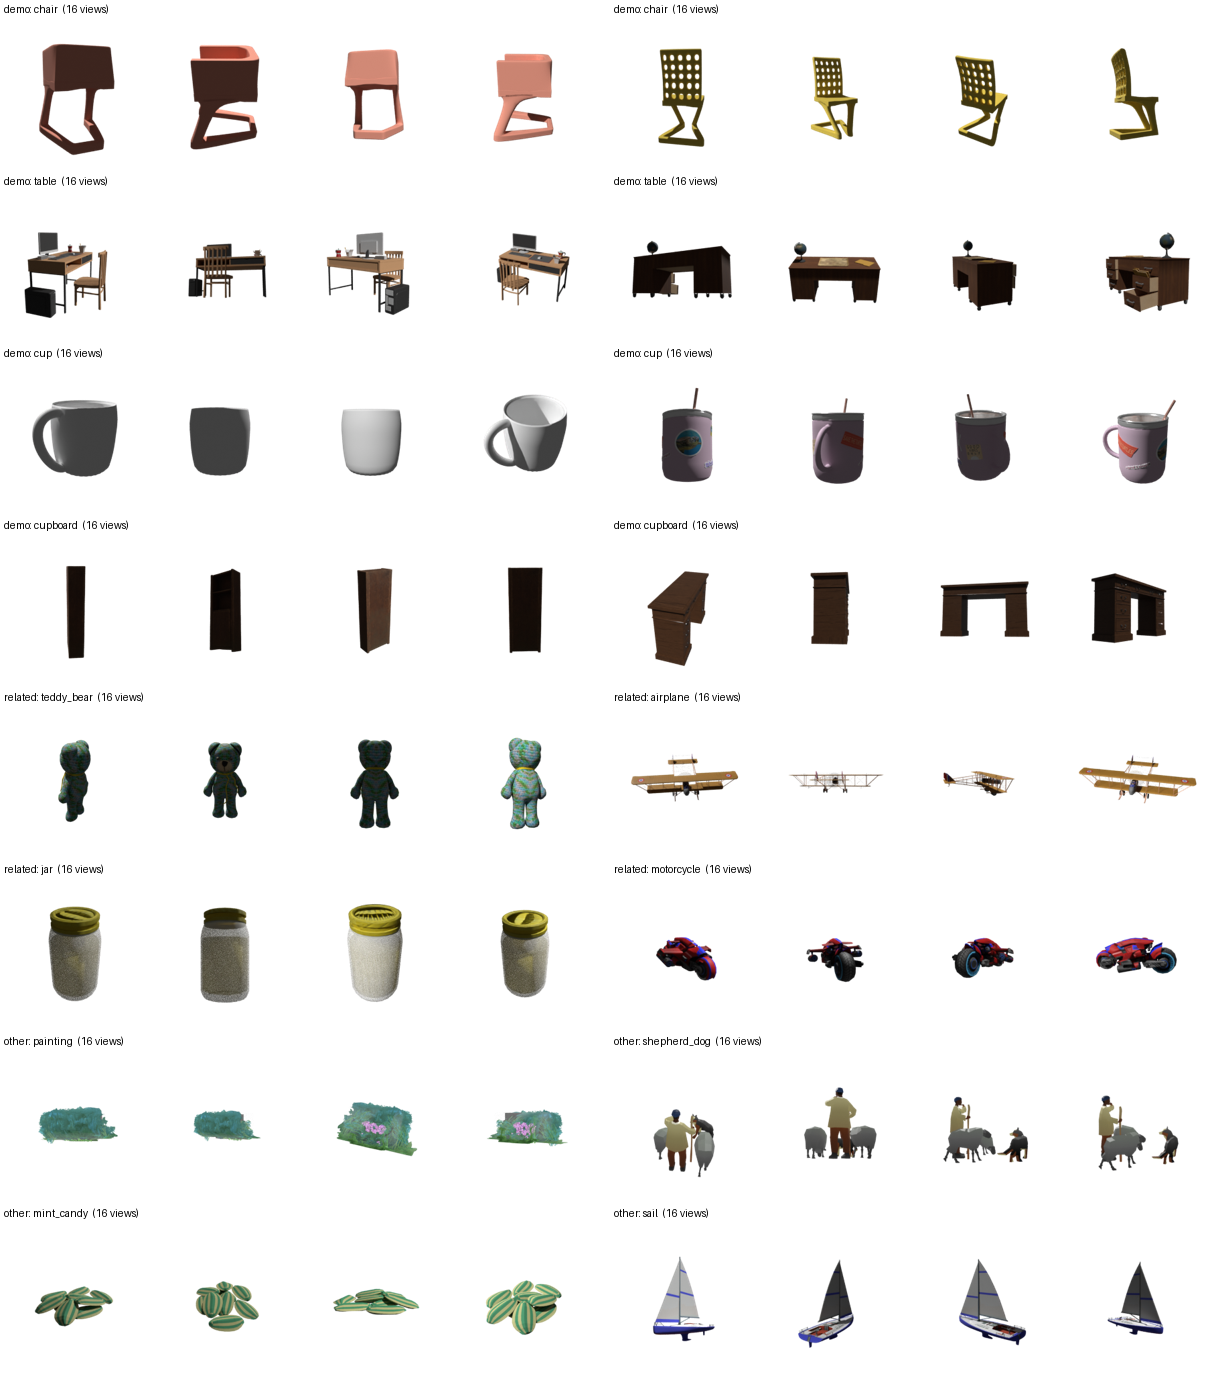
\includegraphics[width=0.85\textwidth]{kaggle_render_check.png}
\caption{Sample Kaggle renders: four of the sixteen views for objects from every group.}
\label{fig:renders}
\end{figure}

\begin{figure}[H]
\centering
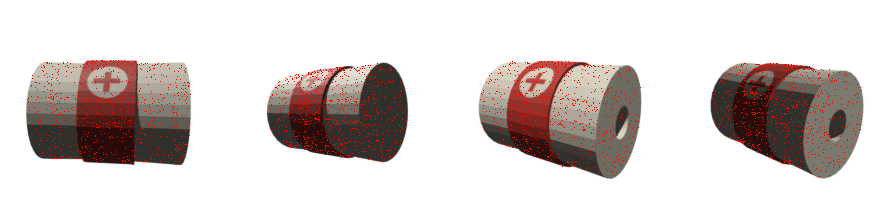
\includegraphics[width=0.85\textwidth]{camera_check.png}
\caption{Camera check: stored 3D surface points (red) projected into four rendered views.}
\label{fig:camera}
\end{figure}

\section{Generator Verification}
Before full training we checked that the generator can learn at all by training it on four objects on a CPU for 700 steps. Validation IoU rose from 0 to 0.67 and texture L1 error fell from 0.29 to 0.06. The extracted meshes have the correct position, size, orientation and colours (Figure~\ref{fig:overfit}); fine parts such as ship masts are still missing, as expected after so few steps.

\begin{figure}[H]
\centering
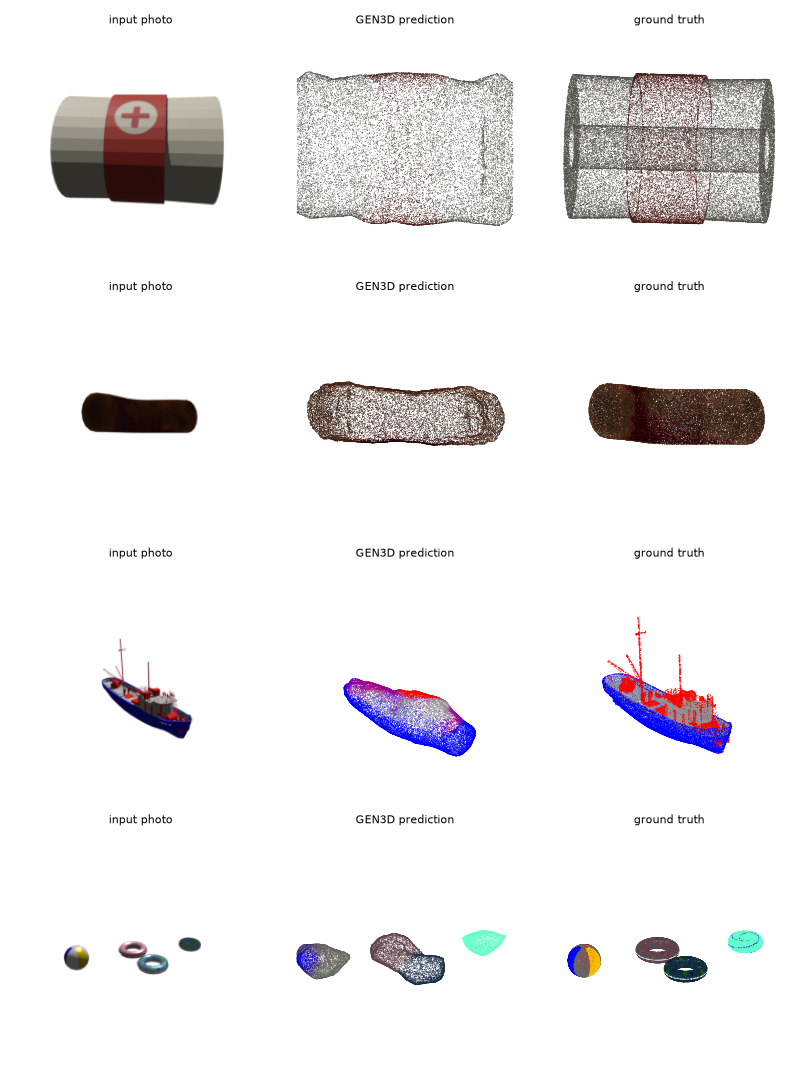
\includegraphics[width=0.7\textwidth]{overfit_check.png}
\caption{Sanity check after 700 steps on four objects: input view, GEN3D prediction and ground truth.}
\label{fig:overfit}
\end{figure}

\section{First Full Training Run (GEN3D-Gen v1)}
GEN3D-Gen v1 was trained on the train split of the 3{,}118 rendered objects (2{,}468 training and 301 validation objects) for 300 epochs on one Kaggle T4 GPU, which took 2.64 hours (about 26\,s per epoch). Validation used a fixed view per object every five epochs; the checkpoint with the best validation IoU was kept.

\begin{table}[H]
\centering
\caption{GEN3D-Gen v1 training summary. IoU is measured on the sampled query points (40\,\% of them close to the surface), so it is stricter than the volumetric IoU reported in \cite{mescheder2019onet} and not directly comparable.}
\label{tab:trainv1}
\begin{tabular}{lcc}
\toprule
 & Train (epoch 300) & Validation (best, epoch 145) \
\midrule
Occupancy IoU & 0.610 & 0.595 \
Total loss & 0.437 & 0.597 \
Colour L1 error & 0.049 & 0.089 \
\bottomrule
\end{tabular}
\end{table}

Figure~\ref{fig:trainv1} shows that the training loss falls steadily, while the validation IoU stops improving after about 35--145 epochs and the validation loss rises after epoch 150. The model starts to memorise the training objects (overfitting), which is expected with only 2{,}468 objects spread over many categories. Figure~\ref{fig:trainv1samples} shows meshes extracted from the best checkpoint: the overall size, pose and main colour are correct, and training objects such as the chair are recognisable, but thin parts (chair legs, masts) are lost and unseen objects come out as smooth blobs.

\begin{figure}[H]
\centering
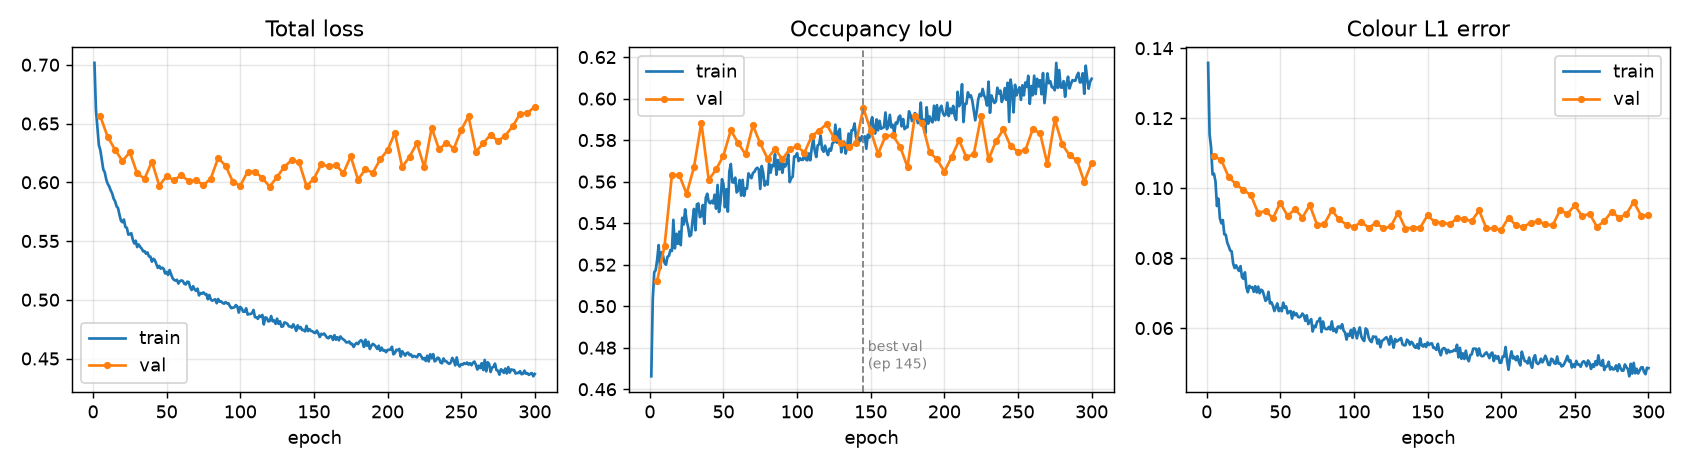
\includegraphics[width=\textwidth]{train_v1_curves.png}
\caption{GEN3D-Gen v1 training curves: total loss, occupancy IoU and colour L1 error for training and validation. The dashed line marks the best validation epoch.}
\label{fig:trainv1}
\end{figure}

\begin{figure}[H]
\centering
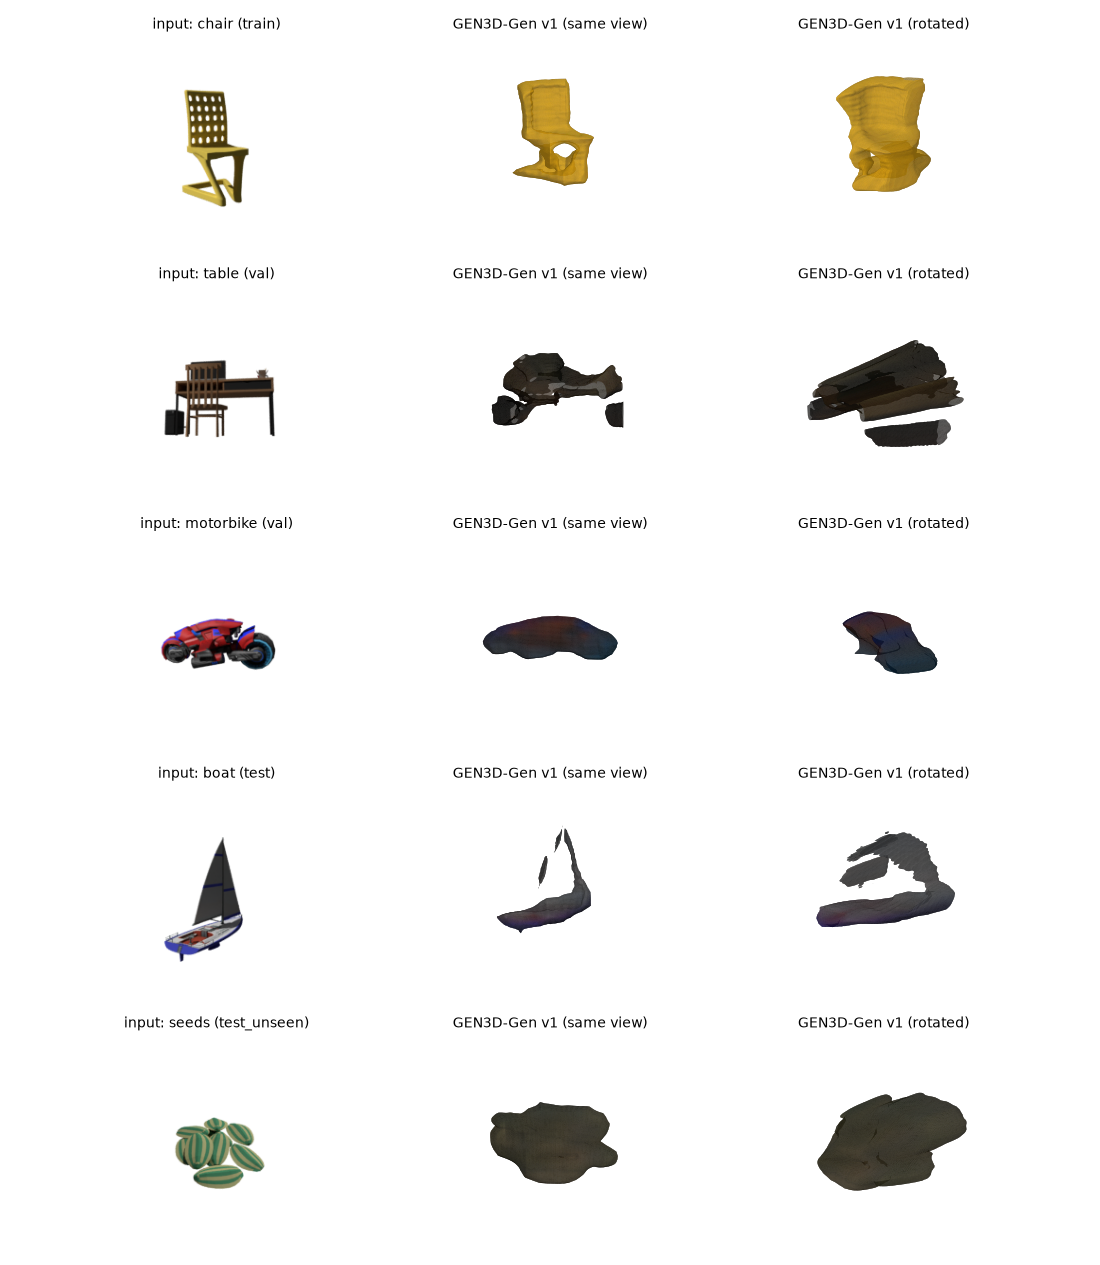
\includegraphics[width=0.85\textwidth]{train_v1_samples.png}
\caption{Meshes generated by GEN3D-Gen v1 (best checkpoint, marching cubes at $128^3$). Labels give the split of each object; only the chair was seen in training.}
\label{fig:trainv1samples}
\end{figure}

\section{Category Fine-Tuning (GEN3D-Gen v1-chair)}
To test whether more focused data helps, v1 was fine-tuned for 200 epochs (0.66\,h on a T4) on the 459 chair, stool and bench training objects, validated on the 54 chair validation objects only. Weight decay (0.05) and colour augmentation ($\pm$15\,\% brightness, contrast and saturation) were switched on. Chair validation IoU rose from 0.602 at the start of fine-tuning to 0.648 at epoch 200 and was still rising; unlike v1, the validation loss did not increase, so the regularisation stopped the overfitting. Figure~\ref{fig:v1chair} compares the two models: the chair model gives cleaner legs and a recognisable seat and back from the side on rendered chairs; on a real photo the front view improves but the depth of the chair is still wrong.

\begin{figure}[H]
\centering
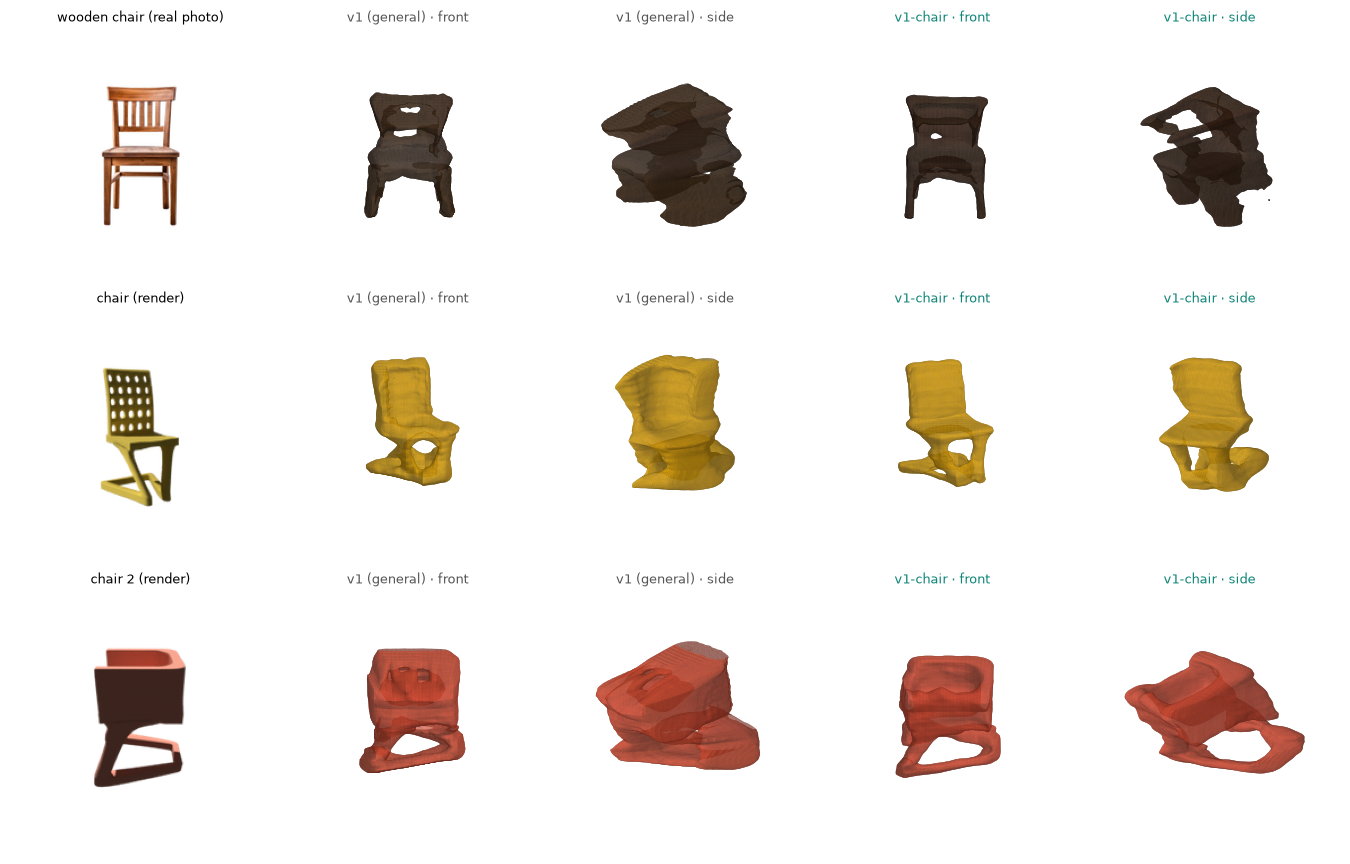
\includegraphics[width=\textwidth]{v1_vs_chair.png}
\caption{GEN3D-Gen v1 (general) vs v1-chair (fine-tuned on chairs) on one real photo and two rendered chairs, front and side views.}
\label{fig:v1chair}
\end{figure}

\section{Second Dataset and Dining-Chair Model (GEN3D-Gen v1-dining)}
Objaverse-LVIS contains only about 520 usable chairs, so we added a second dataset: Amazon Berkeley Objects (ABO)~\cite{collins2022abo}, 7{,}953 real product models with PBR textures, of which 1{,}184 are chairs. The same pipeline (download, checks, our occupancy labels, Blender renders) was extended to read ABO. To focus on one well-defined shape type for the demo, 236 dining chairs (no arms, swivel or bar chairs) were selected by product name and rendered from 24 views each; 235 passed all checks (one was rejected for exceeding 500k faces).

GEN3D-Gen v1-dining was fine-tuned from v1-chair on the 181 training dining chairs for 300 epochs (0.65\,h on a T4). Validation IoU on 27 held-out dining chairs reached 0.698 (epoch 260), with a small gap to the training IoU (0.736). Figure~\ref{fig:dining} shows the effect on a real photograph: from the side the chair now has a seat, an upright back and legs in the right places, and the colour matches the wood.

\begin{figure}[H]
\centering
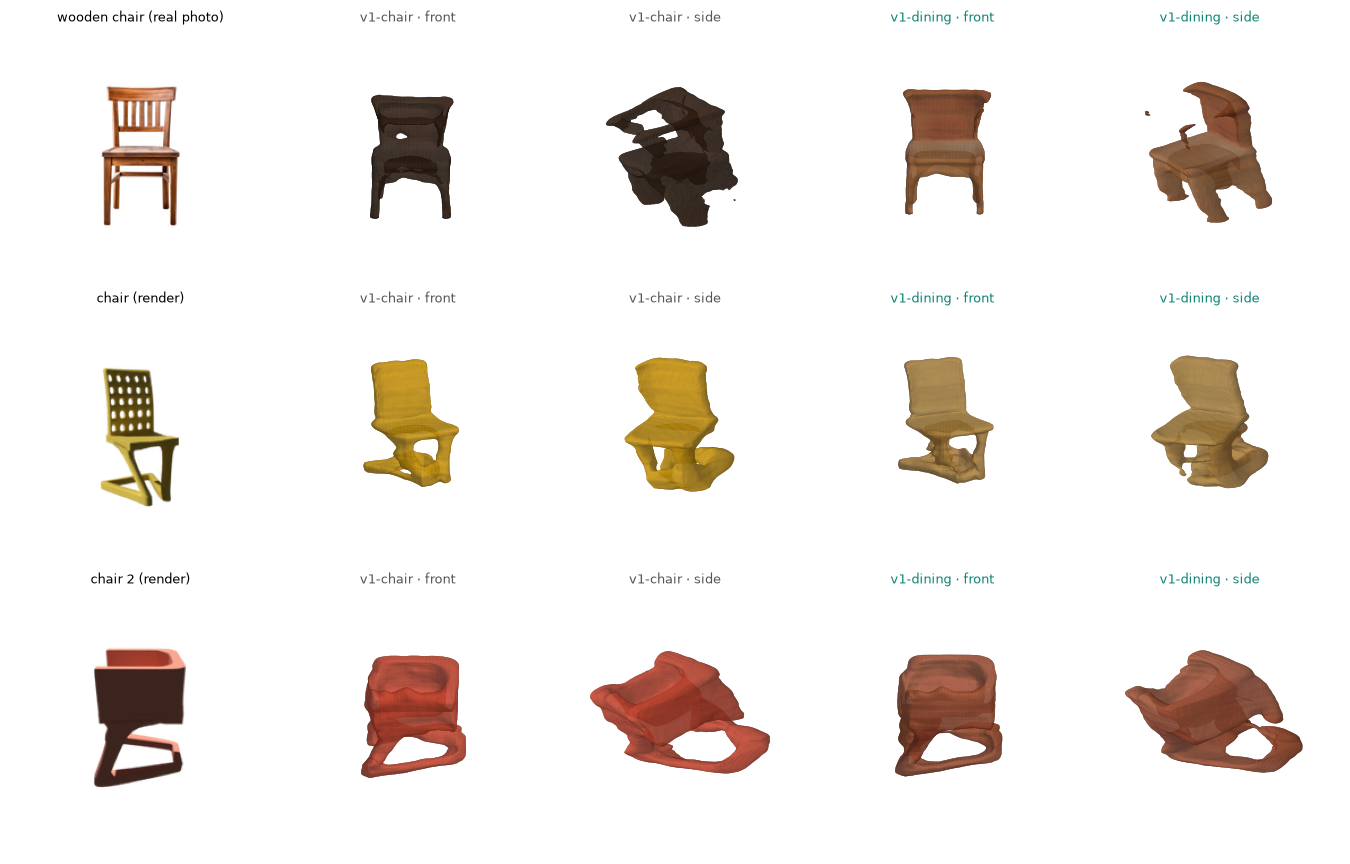
\includegraphics[width=\textwidth]{chair_vs_dining.png}
\caption{v1-chair vs v1-dining on a real photo of a wooden dining chair and two rendered chairs (front and side).}
\label{fig:dining}
\end{figure}

\section{Photo-Projected Colours}
The texture field predicts a smooth average colour, so fine detail such as slats or wood grain is lost. Because the camera of the input photo is known, every mesh vertex can be projected back into the photo. A vertex that faces the camera and is the nearest surface along its pixel (tested with a small z-buffer built from the vertices) takes the photo's pixel colour; hidden vertices keep the texture-field colour, and the two are blended at grazing angles. Figure~\ref{fig:photocol} shows the gain in realism on the visible side at no extra training cost.

\begin{figure}[H]
\centering
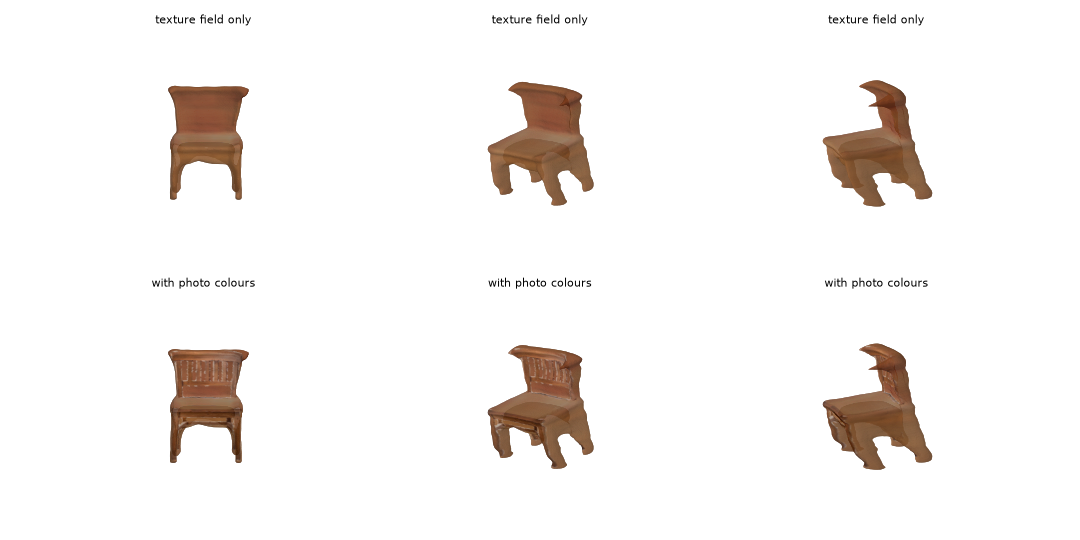
\includegraphics[width=0.9\textwidth]{photo_colours_check.png}
\caption{Same mesh, coloured by the texture field only (top) and with photo-projected colours (bottom).}
\label{fig:photocol}
\end{figure}

\section{Inside the Generator}
To understand where the errors come from, every intermediate result was visualised for one photo (Figure~\ref{fig:inside}): the DINOv2 patch features already separate the back, seat and legs; the front slice of the occupancy field is a clean chair, while the side slice shows the model hedging about the depth of the back (a faint second back on the camera side). This single-view depth ambiguity, not the recognition of the chair, is the main source of error and motivates more aligned training data.

\begin{figure}[H]
\centering
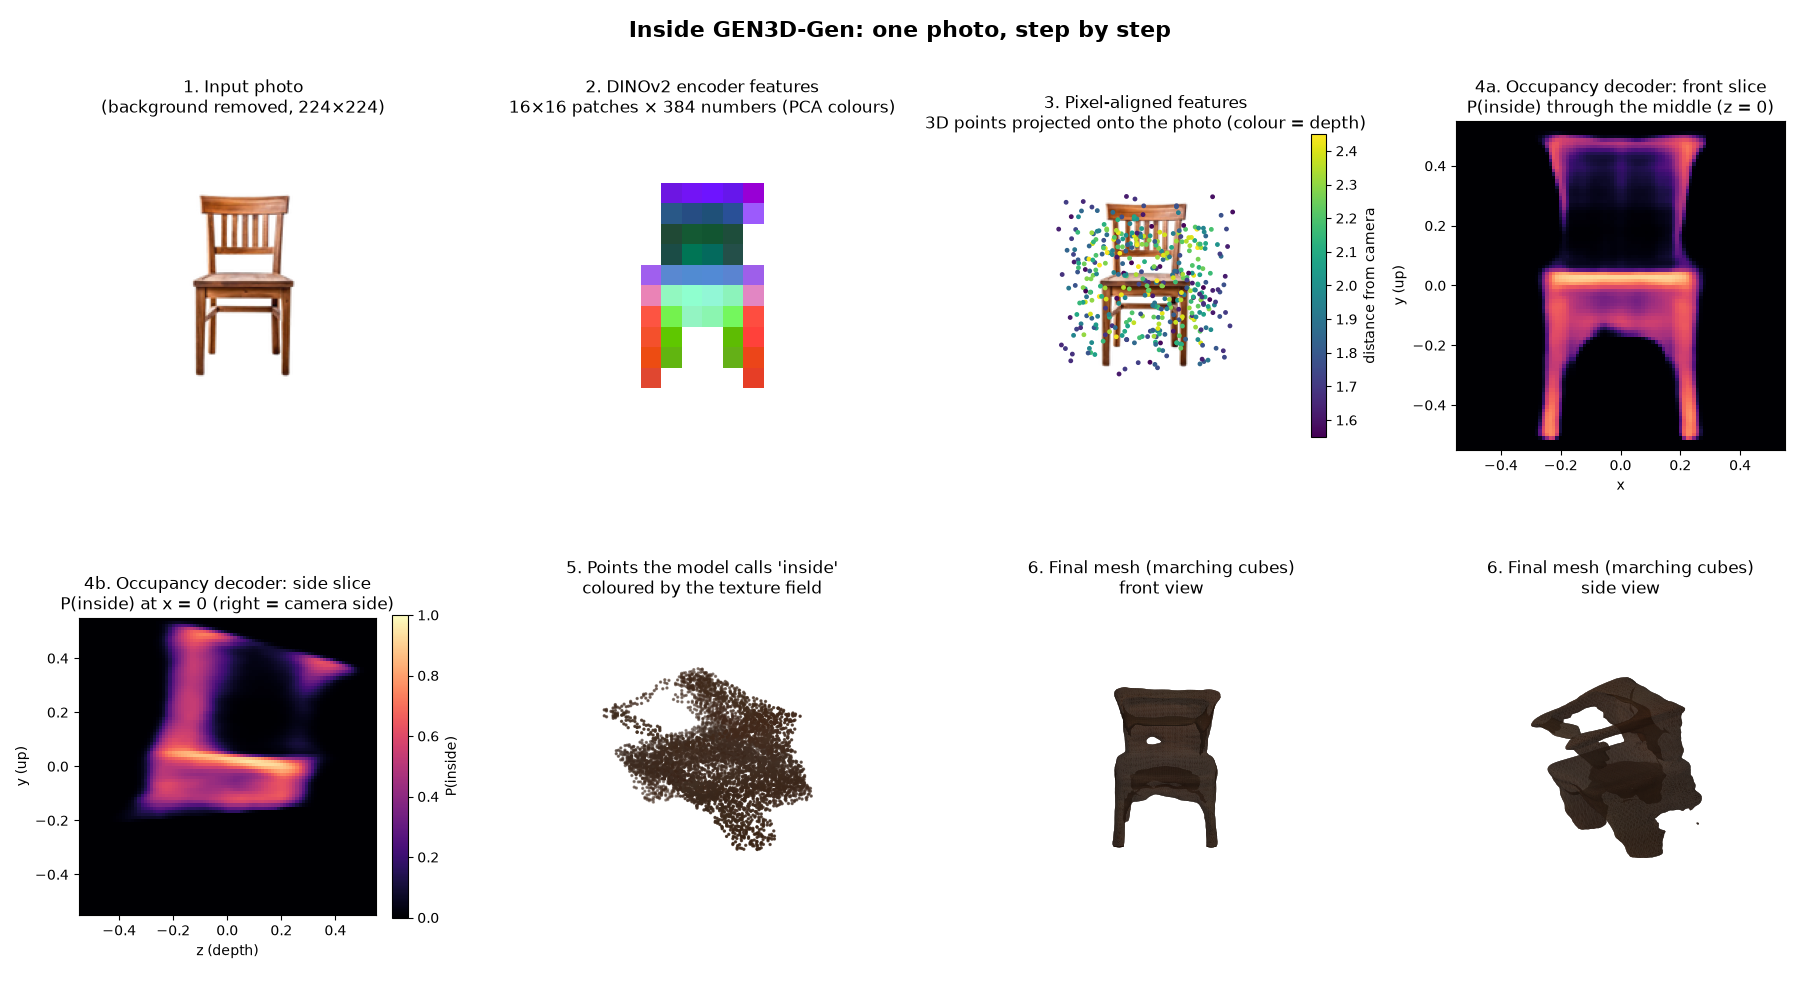
\includegraphics[width=\textwidth]{pipeline_inside.png}
\caption{Internal steps of GEN3D-Gen for one photo: input, encoder features (PCA colours), projected query points, occupancy slices (front and side), inside points with texture-field colours, final mesh.}
\label{fig:inside}
\end{figure}

\section{Following the Occupancy Networks Protocol (GEN3D-Gen v2-chair)}
To compare directly with published work we adopted the data and evaluation protocol of Occupancy Networks~\cite{mescheder2019onet}: the same ShapeNet~\cite{chang2015shapenet} chair objects (6{,}778), the same train/validation/test lists, the same 100k inside/outside points per object and the same 24 renders per object~\cite{choy2016r2n2}. Only the chair byte range (11.4\,GB) of the 73\,GB ONet archive is downloaded; a converter maps the ONet cameras into our convention (verified by projecting the point clouds onto the renders; both datasets turn out to use the same 245-pixel focal length at 224\,px). ShapeNet provides shape but no reliable colour, so this stage trains the shape only and keeps the texture field of v1-dining. Evaluation follows ONet: volumetric IoU on the uniform query points, Chamfer-L1, normal consistency, and F-score at 1\,\%. \todo{v2-chair results table vs ONet Table 1}

\section{Planned Evaluation}
\begin{itemize}[leftmargin=*]
  \item Generator: IoU, Chamfer distance and F-score@1\% on \texttt{test} and \texttt{test\_unseen}, reported per group; ablation of the encoder (DINOv2, ResNet-18 pretrained, ResNet-18 from scratch).
  \item Simplification: at 50\%, 25\% and 10\% of faces, compare PyMeshLab QEM, our QEM and D-QEM using Chamfer and Hausdorff distance (geometry), LPIPS~\cite{zhang2018lpips} and SSIM on multi-view renders (texture), and run time.
\end{itemize}

\chapter{Technical Difficulties and Their Resolution}

\begin{table}[H]
\centering
\caption{Problems met so far and how they were resolved.}
\small
\begin{tabularx}{\textwidth}{rlXX}
\toprule
\# & Module & Problem & Resolution \\
\midrule
1 & Planning & Training a large image-to-3D model needs far more compute than available & Compact occupancy network with a pretrained encoder, trained on Kaggle GPUs \\
2 & Dataset & Only 1{,}283 objects in the four target categories & Class-agnostic training on 1{,}028 categories \\
3 & Dataset & 81\,GB download & 10\,MB cap for non-demo objects: 28\,GB \\
4 & Dataset & Real chairs and tables rejected by the name filter & Removed ``office'', ``kitchen'', ``house'' from the blacklist; 16 objects recovered \\
5 & Download & Files written to the wrong folder on Windows & Own thread-based downloader \\
6 & Preprocess & \texttt{mesh2sdf} does not build on Windows & Own occupancy algorithm \\
7 & Preprocess & Non-watertight meshes & Flood fill from the grid border \\
8 & Preprocess & Shapes inflated by 2.6\% & Exact distances and a $256^3$ grid: 0.4\% \\
9 & Preprocess & 34\,s per object & Bounded nearest-neighbour search: 3\,s \\
10 & Preprocess & Thin objects flagged as hollow & Flag only bulky objects \\
11 & Compute & No local GPU; Colab cannot be automated & Kaggle with API control, chunked and resumable notebooks \\
12 & Rendering & False size warning & Check on real vertices; 100\% camera alignment \\
13 & Compute & Kaggle output too large to download file by file & Keep data on Kaggle; chain notebooks \\
14 & Training & Sanity check stalled at loss 0.6 & More optimisation steps and a higher learning rate for the check \\
15 & Rendering & Runs queued indefinitely & Kaggle retired the P100 default; request T4 explicitly \\
16 & Rendering & 82 objects failed & One crashing Blender process failed its whole shard; worker now restarts and skips only the crashing object \\
17 & Training & v1 overfitted after about 150 epochs (validation loss rising) & Weight decay 0.05 and colour augmentation; fine-tuned models no longer overfit \
18 & Dataset & Only $\sim$520 chairs in Objaverse-LVIS & Added ABO (real product models) and ShapeNet via the ONet data \
19 & Demo & Photos with a printed checkerboard ``transparent'' background & Background mask for light, colourless pixels with small-blob clean-up \
20 & Demo & Upload crashed (RGBA image saved as JPEG) & Keep uploads as PNG \
21 & Rendering & Out-of-memory crash on very large ABO models stopped a run & Retry with fewer workers; skip empty chunks \
22 & Kaggle & Shell pipe inside a training argument (regex with \texttt{|}) & Quote arguments; syntax-check every generated notebook before pushing \
23 & Data & 73\,GB ONet archive & Download only one category's byte range (11.4\,GB for chairs) \
24 & Quality & Mesh colours flat and blurry & Project the photo onto the visible side of the mesh \\
\bottomrule
\end{tabularx}
\end{table}

\chapter{Project Management}

\section{Timeline}
\begin{table}[H]
\centering
\caption{FYP-1 timeline and status.}
\small
\begin{tabularx}{\textwidth}{lXl}
\toprule
Phase & Work & Status \\
\midrule
Planning & Architecture, dataset decision, rubric mapping & Done \\
Data & Selection, download, checks, preprocessing (7{,}467 objects) & Done \\
Rendering & 16 views per object on Kaggle GPU & 3{,}118 done; rest scheduled \\
Generator & Model, dataset loader, training, extraction & Implemented; training v1 \\
Simplification & UV-aware QEM & Next \\
Demo & Gradio interface & Next \\
Documentation & Diagrams, SRS, test plan, report & In progress \\
\bottomrule
\end{tabularx}
\end{table}
\todo{add Gantt chart with dates}

\section{Work Distribution}
\todo{fill in names per phase: requirements, design, implementation, testing, documentation}

\section{Supervisor Meetings}
\todo{summarise weekly meetings from docs/meetings.md}

\section{Risks}
\begin{table}[H]
\centering
\caption{Risks and mitigations.}
\small
\begin{tabularx}{\textwidth}{XX}
\toprule
Risk & Mitigation \\
\midrule
Limited GPU quota (30\,h/week) & Demo objects rendered first; resumable notebooks; schedule around weekly reset \\
Poor results on real photographs & Background removal, random backgrounds and lighting in training, DINOv2 encoder \\
Noisy Objaverse labels and multi-object scenes & Class-agnostic training; visual review before the final run \\
Duplicates between train and test & Embedding-based de-duplication before final evaluation \\
Blurry texture & Project visible texture from the input image; texture baking \\
\bottomrule
\end{tabularx}
\end{table}

\chapter{Conclusion and Future Work}

\section{Conclusion}
In the first part of the project we built the data foundation and the generator of GEN3D. A class-agnostic dataset of 7{,}467 clean objects from 1{,}028 Objaverse-LVIS categories was curated, labelled with our own occupancy method and rendered with calibrated cameras. The generator, a DINOv2-based occupancy network with pixel-aligned features and a texture field, is implemented and has been shown to learn shape and colour. All heavy computation runs reproducibly on Kaggle under API control.

\section{Future Work}
\begin{itemize}[leftmargin=*]
  \item Finish rendering the remaining objects and train the generator on the full dataset.
  \item Implement the UV-aware QEM and compare it with PyMeshLab.
  \item Build the Gradio demo.
  \item FYP-2: train the D-QEM Transformer, add UV unwrapping and texture baking, run the full evaluation and ablations.
\end{itemize}


\bibliographystyle{IEEEtran}
\bibliography{references}

\end{document}
